\documentclass[tikz,border=10pt]{standalone}
\usepackage{tikz}
\usetikzlibrary{arrows.meta, positioning, shapes.geometric, decorations.pathreplacing, calc, fit}

\begin{document}
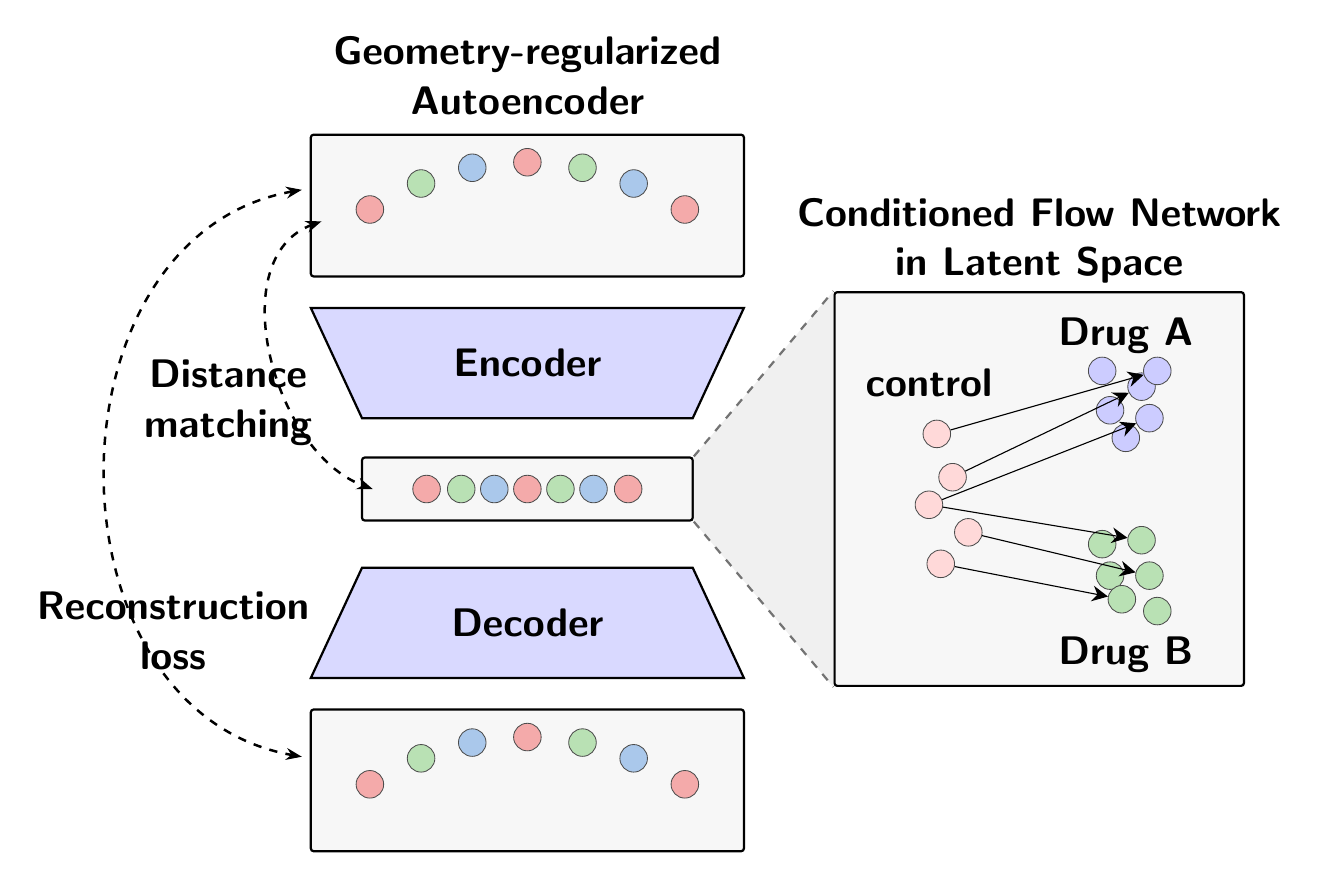
\begin{tikzpicture}[
    font=\sffamily\fontsize{15}{18}\selectfont,
    dashbox/.style={draw, thick, rounded corners=1pt, inner sep=6pt, fill=black!3},
    trapfont/.style={font=\sffamily\bfseries\fontsize{15}{18}\selectfont},
    thickarrow/.style={-{Stealth[length=4mm,width=5mm]}, line width=2.8mm, draw=black!45},
    thinarrow/.style={-{Stealth[length=2mm,width=2mm]}, line width=0.4pt, draw=black},
    pink/.style={circle, draw=black!70, line width=0.3pt, fill=red!15, minimum size=3.5mm, inner sep=0pt},
    blue/.style={circle, draw=black!70, line width=0.3pt, fill=blue!20, minimum size=3.5mm, inner sep=0pt},
    green/.style={circle, draw=black!70, line width=0.3pt, fill=mG, minimum size=3.5mm, inner sep=0pt},
    mdot/.style={circle, draw=black!70, line width=0.3pt, minimum size=3.5mm, inner sep=0pt},
]

% Each dot is one of red / green / blue (pastel); same ordering on top arc and bottom row
\definecolor{mR}{RGB}{244,170,170}
\definecolor{mG}{RGB}{185,225,180}
\definecolor{mB}{RGB}{170,200,235}

% ===== LEFT: Encoder/Decoder =====
% Encoder trapezoid (wide top = 55mm matches data box; narrow bottom = 42mm matches latent)
\draw[fill=blue!15, thick]
    (-2.75, 2.9) -- (2.75, 2.9) -- (2.1, 1.5) -- (-2.1, 1.5) -- cycle;
\node[trapfont] (enc) at (0, 2.2) {Encoder};

% Curved data manifold box — width matches top (wide side) of encoder (55mm)
\node[dashbox, inner sep=0, minimum width=55mm, minimum height=18mm] (datab) at (0,4.2) {};
\foreach \c/\x/\y in {mR/-2.0/-0.05, mG/-1.35/0.28, mB/-0.7/0.48, mR/0/0.55, mG/0.7/0.48, mB/1.35/0.28, mR/2.0/-0.05} {
    \node[mdot, fill=\c] at ($(datab.center) + (\x,\y)$) {};
}

% Latent box: width matches the narrow end of encoder (bottom) / decoder (top)
\node[dashbox, minimum width=42mm, minimum height=8mm] (latb) at (0,0.6) {};
\foreach \c/\i in {mR/-3.2, mG/-2.1, mB/-1.05, mR/0, mG/1.05, mB/2.1, mR/3.2} {
    \node[mdot, fill=\c] at ($(latb) + (\i*4mm,0)$) {};
}
\coordinate (latb-east) at (latb.east);
\coordinate (latb-west) at (latb.west);
\coordinate (latb-ne) at (latb.north east);
\coordinate (latb-se) at (latb.south east);

% Decoder trapezoid (narrow top = 42mm matches latent; wide bottom = 55mm matches recon)
\draw[fill=blue!15, thick]
    (-2.1, -0.4) -- (2.1, -0.4) -- (2.75, -1.8) -- (-2.75, -1.8) -- cycle;
\node[trapfont] (dec) at (0, -1.1) {Decoder};

% Distance matching: dashed double-ended arrow between data box and latent box (left side)
\draw[{Stealth[length=2mm]}-{Stealth[length=2mm]}, line width=0.9pt, dashed]
    ($(datab.west) + (0.15,-0.2)$)
    to[out=-160, in=160]
    ($(latb-west) + (0.15,0)$);

% Label "Distance matching"
\node[font=\sffamily\bfseries\fontsize{15}{18}\selectfont, align=center] at (-3.8, 1.7) {Distance\\matching};

% Reconstructed manifold — width matches bottom (wide side) of decoder
\node[dashbox, inner sep=0, minimum width=55mm, minimum height=18mm] (recb) at (0,-3.1) {};
\foreach \c/\x/\y in {mR/-2.0/-0.05, mG/-1.35/0.28, mB/-0.7/0.48, mR/0/0.55, mG/0.7/0.48, mB/1.35/0.28, mR/2.0/-0.05} {
    \node[mdot, fill=\c] at ($(recb.center) + (\x,\y)$) {};
}

% Reconstruction loss: double-headed dashed arrow on the far-left, spanning
% the full AE from original data (top) down to reconstruction (bottom).
\draw[{Stealth[length=2mm]}-{Stealth[length=2mm]}, line width=0.9pt, dashed]
    ($(datab.west) + (-0.1,0.2)$)
    to[out=-170, in=170, looseness=1.2]
    ($(recb.west) + (-0.1,0.3)$);

\node[font=\sffamily\bfseries\fontsize{15}{18}\selectfont, align=center] at (-4.5, -1.2) {Reconstruction\\loss};

% Title
\node[font=\sffamily\bfseries\fontsize{15}{18}\selectfont, align=center] at (0, 5.85) {Geometry-regularized\\Autoencoder};

% ===== Map-inset style expansion from latent box to ODE box =====
\begin{scope}[yshift=-0.6cm, xshift=-1.3cm]
\node[dashbox, minimum width=52mm, minimum height=50mm] (odebox) at (7.8, 1.2) {};

% Light filled trapezoid connecting latent box (source) to ODE box (destination)
\fill[black!6]
    (latb-ne) --
    ($(odebox.north west)$) --
    ($(odebox.south west)$) --
    (latb-se) -- cycle;

% Dashed guide lines indicating the expansion (like an inset map magnifier)
\draw[dashed, thick, black!55] (latb-ne) -- ($(odebox.north west)$);
\draw[dashed, thick, black!55] (latb-se) -- ($(odebox.south west)$);

% ===== RIGHT: ODE latent space =====
% Control (pink) cluster - left middle
\coordinate (c1) at (6.5, 1.9);
\coordinate (c2) at (6.7, 1.35);
\coordinate (c3) at (6.4, 1.0);
\coordinate (c4) at (6.9, 0.65);
\coordinate (c5) at (6.55, 0.25);

\node[pink] (cA) at (c1) {};
\node[pink] (cB) at (c2) {};
\node[pink] (cC) at (c3) {};
\node[pink] (cD) at (c4) {};
\node[pink] (cE) at (c5) {};

% Drug A cluster (blue, top right)
\coordinate (bA) at (8.9, 2.4);
\node[blue] (a1) at (8.6, 2.7) {};
\node[blue] (a2) at (9.1, 2.5) {};
\node[blue] (a3) at (8.7, 2.2) {};
\node[blue] (a4) at (9.2, 2.1) {};
\node[blue] (a5) at (8.9, 1.85) {};
\node[blue] (a6) at (9.3, 2.7) {};

% Drug B cluster (green, bottom right)
\node[green] (g1) at (8.6, 0.5) {};
\node[green] (g2) at (9.1, 0.55) {};
\node[green] (g3) at (8.7, 0.1) {};
\node[green] (g4) at (9.2, 0.1) {};
\node[green] (g5) at (8.85, -0.2) {};
\node[green] (g6) at (9.3, -0.35) {};

% Arrows from control to Drug A
\draw[thinarrow] (cA) -- (a6);
\draw[thinarrow] (cB) -- (a2);
\draw[thinarrow] (cC) -- (a4);

% Arrows from control to Drug B
\draw[thinarrow] (cC) -- (g2);
\draw[thinarrow] (cD) -- (g4);
\draw[thinarrow] (cE) -- (g5);

% Labels
\node[font=\sffamily\bfseries\fontsize{15}{18}\selectfont] at (8.9, 3.15) {Drug A};
\node[font=\sffamily\bfseries\fontsize{15}{18}\selectfont] at (8.9, -0.9) {Drug B};
\node[font=\sffamily\bfseries\fontsize{15}{18}\selectfont] at (6.4, 2.55) {control};

% Title
\node[font=\sffamily\bfseries\fontsize{15}{18}\selectfont, align=center] at (7.8, 4.35) {Conditioned Flow Network\\in Latent Space};
\end{scope}

\end{tikzpicture}
\end{document}
